\chapter{Method Description}

In this section, the origin DOI method, JDOI method and approximation method based on DOI method are described. In section \ref{sec: 2.1},, we introduce the origin DOI method, see\cite{heath_monte_nodate}. In section \ref{sec: 2.2}, we illustrate the approximation method proposed by \cite{kristensen_adding_2011}. In section \ref{sec: 2.3}, we discuss our estimator to price American options based on JDOI method, \cite{auster_jdoi_2021}.

\section{The DOI Variance Reduction Method}
\label{sec: 2.1}

Consider a multi-factor model, in which a $d$-dimensional vector of state variables $X(t)$ on a filtered probability space$(\Omega,\mathcal F, \mathbb Q)$ satisfies the following Stochastic Differential Equations(SDEs)

\begin{equation}\label{general model}
    dX(t) = \mu(t, X(t)) dt + \sigma(t, X(t)) dW(t)
\end{equation}

\noindent where $\mu(t,X(t))$ and $\sigma(t, X(t))$ are drift and diffusion functions under the risk-neutral measure $\mathbb Q$, which also satisfies appropriate growth and Lipschiz conditions such that equation(\ref{general model}) admits a unique strong solution and is Markovian; $W(t)$ is a $d$-dimensional standard Brownian Motion and $t \in [0,T]$.

% Besides, we also need to consider the stopping time formulation such that we can apply DOI method to path-dependent options, we shall discuss it later in section \ref{sec: 2.3} when pricing American options.

% Let $G(t, x)$ be the payoff function of derivatives written on $X(t)$ and current state $X(t) = x$, $t\in[0,T]$, assume $G(t,x)$ satisfies that 

% \begin{equation}
%     \mathbb{E}_{t, x}\left[\sup _{0 \leq u \leq T-t}\left|e^{-\int_t^{t+u} R(s,X(s)) ds} G(T, X(t+u))\right|\right]<\infty
% \end{equation}

% \begin{equation}
%     V(t,x) = \mathbb{E}^{t,x}[e^{-\int_t^T R(s,X(s)) ds} G(T, X(T))]
% \end{equation}

Let $V(t,x)$ be the value function of European option written on $X(T)$ with current state $X(t)=x$, $G(t, x)$ be the payoff function. We define the infinitesimal generator $\mathcal{L}$ associated with equation(\ref{general model})to be

\begin{equation}\label{general inf gen}
    \begin{aligned}
        (\mathcal{L} V)(t, x)&=\frac{\partial V}{\partial t} + \sum_{i=1}^{d} \mu_i(t, x) \frac{\partial V}{\partial x}+\frac{1}{2} \sum_{i=1}^{d}\sum_{j=1}^{d} (\sigma(t,x) \sigma^{\intercal}(t,x))_{i,j} \frac{\partial^2 V}{\partial x_i x_k}
    \end{aligned}
\end{equation}

Let $R(t,x)$ be the instantaneous short-term interest rate, combining with equation(\ref{general model}) and equation(\ref{general inf gen}), the price of European option $V$ is a solution to the following partial differential equation(PDE)

\begin{equation}\label{pde under general}
    \mathcal{L}V(x,t) = R(x,t)V(x,t)
\end{equation}
\noindent with boundary condition $V(T,x(T)) = G(T,X(T))$. It's easily seen that under risk neutral measure $\mathbb Q$, the instantaneous option price change is equal to the price gain in saving account. 

Next we consider to use a $m$-dimensional($m \leq d$) process $\bar{X}(t)$ which is a simpler auxiliary model to approximate the price of option. $\bar{X}(t)$ satisfies the following SDE

\begin{equation}\label{approx model}
    \begin{aligned}
        &d\bar{X}(t)= \begin{cases}   \bar{\mu}_i(t, \bar{X}(t)) dt + \bar{\sigma}_i(t, \bar{X}(t)) dW(t) & 1 \leq i \leq m \\
        \bar{\mu}_i(t, \bar{X}(t))=0, \ \bar{\sigma}_i(t, \bar{X}(t))=0 & m < i \leq d \end{cases}
        \end{aligned}
\end{equation}

\noindent where $\bar{\mu}(t, \bar{X}(t))$ and $\bar{\sigma}(t, \bar{X}(t))$ are drift and diffusion functions, and they are also assumed to satisfy appropriate conditions such that equation(\ref{approx model}) admits a unique strong solution and is Markovian.

Let $\bar{V}(t,x)$ be the option price written on process $\bar{X}(t)$ and assume $\bar{V}$ has closed form solution under this new process, the infinitesimal generator $\bar{\mathcal{L}}$ for option price $\bar{V}$ is the same as equation(\ref{general inf gen}) but replacing $\mu(t,x)$, $\sigma(t,x)$ by $\bar{\mu}(t,x)$ and $\bar{\sigma}(t,x)$. Therefore $\bar{V}(t,x)$ is a solution to

\begin{equation}\label{pde under approx}
    \mathcal{\bar{L}}\bar{V}(x,t) = R(x,t)\bar{V}(x,t)
\end{equation}



Denote the price difference $\Delta V(t,x) = V(t,x) - \bar{V}(t,x)$, by subtract equation(\ref{pde under approx} from equation(\ref{pde under general})), $\Delta V(t,x)$ satisfies the following equation

\begin{equation}
    \mathcal{L} \Delta V(t, x)+ (\mathcal{L}-\bar{\mathcal{L}}) V(t,x)=R(x, t) \Delta V(t, x)
\end{equation}

\noindent with boundary condition $\Delta V(T,x) = G(T,x) - \bar{G}(T,x)$. We can find that the price difference arises from two parts:

\begin{itemize}
    \item The use of a wrong payoff function $\bar{G}(t,x)$, it can be eliminated once we use the same payoff function in auxiliary model as it in general model
    \item The discrepancies between the auxiliary model and general model.
\end{itemize}

\noindent Define $\delta(t,x) = (\mathcal{L}-\bar{\mathcal{L}}) V(t,x)$, $d(t,x) = G(t,x) - \bar{G}(t,x)$, under standard regularity conditions\footnote{See Appendix A in \cite{kristensen_adding_2011}}, we can derive the following formula by using Feynman-Kac representation

\begin{equation}\label{feynman-kac rep}
    \begin{gathered}
        V(t, x)=\bar{V}(t,x)+\mathbb{E}_{t,x}\left[\exp \left(-\int_{t}^{T} R(s,X(s)) d s\right) d(T,X(T))\right] \\
        \quad+\int_{t}^{T} \mathbb{E}_{t,x}\left[\exp \left(-\int_{t}^{s} R(u, X(u)) d u\right) \delta(s,X(s))\right] d s
        \end{gathered}
\end{equation}

Finally, under the initial condition $Z_0 = V(0,x)$, the DOI estimator

\begin{equation}
    \begin{gathered}
        Z_t =\bar{V}(t, x)+\exp \left(-\int_{t}^{T} R(s,X(s)) d s\right) d(T,X(T)) \\
        \quad+\int_{t}^{T} \exp \left(-\int_{t}^{s} R(x(u), u) d u\right) \delta(s,X(s))d s
        \end{gathered}
\end{equation}

\noindent is an unbiased estimator for $Z_0$. And if a good auxiliary model is chosen,  the variance of $Z_t$ will be small.
% With this new process, the European option written on $\bar{X}(t)$ is given by

% \begin{equation}
%     \bar{V} = \mathbb{E}_{t, x}\left[e^{-\int_t^{t+u} R(s,\bar{X}(s)) ds} G(T, \bar{X}(t+u))\right]
% \end{equation}

% \noindent and assume the following additional integrability condition

% \begin{equation}
%     \mathbb{E}_{t, x}\left[\sup _{0 \leq u \leq T-t}\left|e^{-\int_t^{t+u} R(s,\bar{X}(s)) ds} G(T, \bar{X}(t+u))\right|\right]<\infty
% \end{equation}

% Additionally, strong Markovian arguments imply that the European-style option $\bar{V}$ satisfies

% \begin{equation}
%     L\bar{V}(x,t) + q(t,x) = R(x,t)\bar{V}(x,t)
% \end{equation}



\section{Approximation Method based on DOI method}
\label{sec: 2.2}

Recall equation\eqref{feynman-kac rep}, instead of using it as an estimator to do simulations, \cite{kristensen_adding_2011} make some additional assumptions and use Ito-Taylor expansion to get closed form approximation formula.

For sufficiently smooth function $f(t,x), $Ito-Taylor expansion is given by

\begin{equation}
    \mathbb{E}^{t, x}[f(s, X(s))]=\sum_{N=0}^{J} \frac{(s-t)^{N}}{N !}\left(\mathcal{L}\right)^{N} f(t, x)+\mathcal{R}_{J}
\end{equation}

\noindent where the remainder term $\mathcal{R}_{J}$ is given by

\begin{equation}
    \mathcal{R}_{J}=\mathbb{E}^{t, x}\left[\int_{t}^{s} d u_{1} \int_{t}^{u_{1}} d u_{2} \cdots \int_{t}^{u_{J}}\left(\mathcal{L}\right)^{J+1} f\left(u_{J+1}, X\left(u_{J+1}\right)\right) d u_{J+1}\right]
\end{equation}

The process $X(t)$ here is defined in equation\eqref{general model}, and the infinitesimal generator $\mathcal{L}$ is defined in equation\eqref{general inf gen}.

Assume closed form solution of option price $\bar{V}$ under auxiliary model and the difference of payoff function $d(t,x)$ is sufficiently smooth. In other words, for $N \geq 1$, assume $\delta(t,x)$ and $d(t,x)$ to be $2N$ times differentiable with respect to $x$, $\delta(t,x)$ to be $N$ times differentiable with respect to $t$. By applying Ito-Taylor expansion to equation\eqref{feynman-kac rep}

\begin{equation}
    \begin{gathered}
        V(t, x)=\bar{V}(t,x)+\mathbb{E}_{t,x}\left[\exp \left(-\int_{t}^{T} R(s,X(s)) d s\right) d(T,X(T))\right] \\
        \quad+\int_{t}^{T} \mathbb{E}_{t,x}\left[\exp \left(-\int_{t}^{s} R(u, X(u)) d u\right) \delta(s,X(s))\right] d s
        \end{gathered}
\end{equation}

\noindent We can get a closed-form approximation formula

\begin{equation}\label{approx formula}
    V_{N}(t, x)=\bar{V}(t,x)+\sum_{n=0}^{N} \frac{(T-t)^{n}}{n !} d_{n}(t, x)+\sum_{n=0}^{N} \frac{(T-t)^{n+1}}{(n+1) !} \delta_{n}(t, x)
\end{equation}

\noindent where $d_0(t,x)=d(x)$, $\delta_0(t,x)=\delta(t,x)$, and

\begin{equation}
    \begin{aligned}
        &d_{n}(t, x)=L d_{n-1}(t, x)-R(t, x) d_{n-1}(t, x) \\
        &\delta_{n}(t, x)=L \delta_{n-1}(t, x)-R(t, x) \delta_{n-1}(t, x)
        \end{aligned}
\end{equation}

Note that the terms in equation(\eqref{approx formula}) can be calculated once for all, meaning that it be computed much faster than simulation methods using estimator.

\section{JDOI method}
\label{sec: 2.3}
  
\normalsize 

% \begin{figure}[htp]
% \centering
% 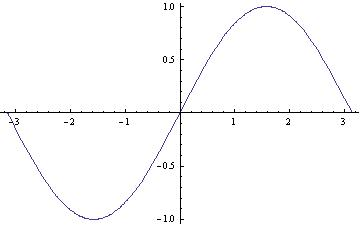
\includegraphics{sin_x.jpg}
% \caption{Transverse momentum distributions}\label{fig:erptsqfit}
% \end{figure}

